\clearpage
\section{Nízkošumový selektivní zesilovač}
%\subsection{Popis funkce obvodu}
\indent\indent Tento obvod má za úkol zesílit vstupní signál a současně odstranit nežádoucí signál mimo přijímané pásmo. Vstupní signál z antény je přiváděn konektorem P1, dále pokračuje k transformátoru T1. Ten slouží jako impedanční přizpůsobení, kdy upravuje  impedanci ze vstupních $50~\Omega$ směrem nahoru až na několik set ohmů. Impedance závisí na kmitočtu vstupního signálu. Sekundární vinutí transformátoru T1 tvoří s kondenzátorem C2 a kapacitním trimrem C3 paralelní rezonanční obvod naladěný na frekvenci $14~MHz$. Tento rezonanční obvod je spojen kapacitní vazbou, kterou tvoří kondenzátor C4 s dalším paralelním rezonančním obvodem. Ten je tvořen kondenzátorem C5, kapacitním trimrem C6 a primárním vinutím transformátoru T2. Tento rezonanční obvod je naladěný na frekvenci $14,35~MHz$. Další funkce transformátoru T2 je transformace impedance zpátky na $50~\Omega$. Transformátory T1 a T2 jsou navinuty na toroidním jádru Amidon T44-2. Upravený signál pokračuje dále přes vazební kondenzátor do tranzistorového zesilovače. Jedná se o zesilovač pracující ve třídě A a je postavený s tranzistorem KF630D. Teplotní stabilizaci zajišťuje záporná proudová zpětná vazba tvořená rezistory R3 a R4. Napětí báze je stabilizováno  zápornou napěťovou zpětnou vazbou tvořenou rezistory R1, R2 a R5. Výstupní proud z tranzistoru teče do bifilárně navinutého transformátoru T3. T3 tvoří sedm závitů izolovanou dvoulinkou drátu průměru $0,8~mm$ na toroidní jádro z materiálu N2. Tento transformátor přizpůsobuje výstupní impedanci na $50~\Omega$. Před výstupním konektorem je ještě zařazen kondenzátor C11, který slouží k oddělení stejnosměrné složky. Celý obvod se tedy chová jako aktivní frekvenční propust.

%\subsection{Frekvenční propust}
%\indent\indent 
%Jak již bylo zmíněno výše, jedná se o dva paralelní rezonanční obvody. Jeden je naladěný na $14.00~MHz$ a druhý na $14.35~MHz$, což odpovídá šířce přijímaného pásma. Transformátory jsou navinuty na toroidní jádra materiálu Amidon T-44-2. Oba transformátory jsou navinuty stejně. Rezonanční cívku tvoří 27 závitů měděným drátkem průměru $0.3~mm$. $50~\Omega$ výstup je navinut třemi závity měděného drátu průměru $0.8~mm$.

% selektivita
\begin{figure}[H]
	\centering
	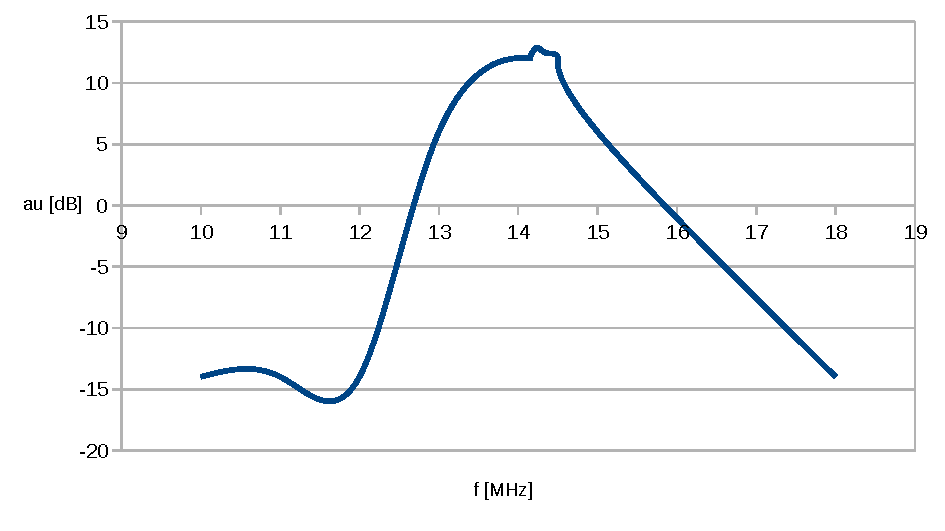
\includegraphics[width=170mm]{img/LNA/sel.pdf}
	\caption{Graf selektivnosti aktivní pásmové propusti}    		
\end{figure}

% schéma
\begin{landscape}
	\begin{figure}[h]
		\centering 	
		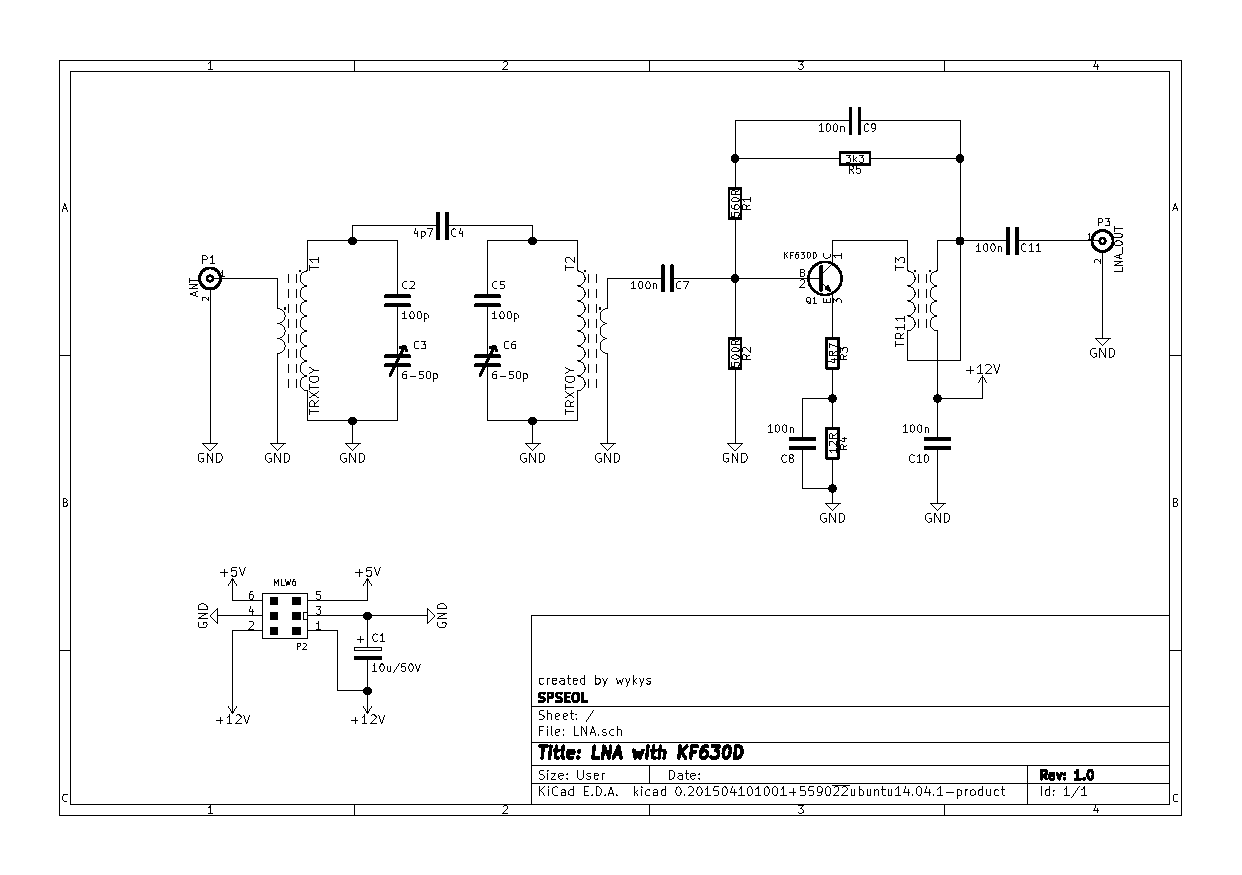
\includegraphics[height=\textwidth]{img/LNA/sch.pdf}
		\caption{Schéma zapojení nízkošumového selektivního zesilovače}	
	\end{figure}
\end{landscape}
%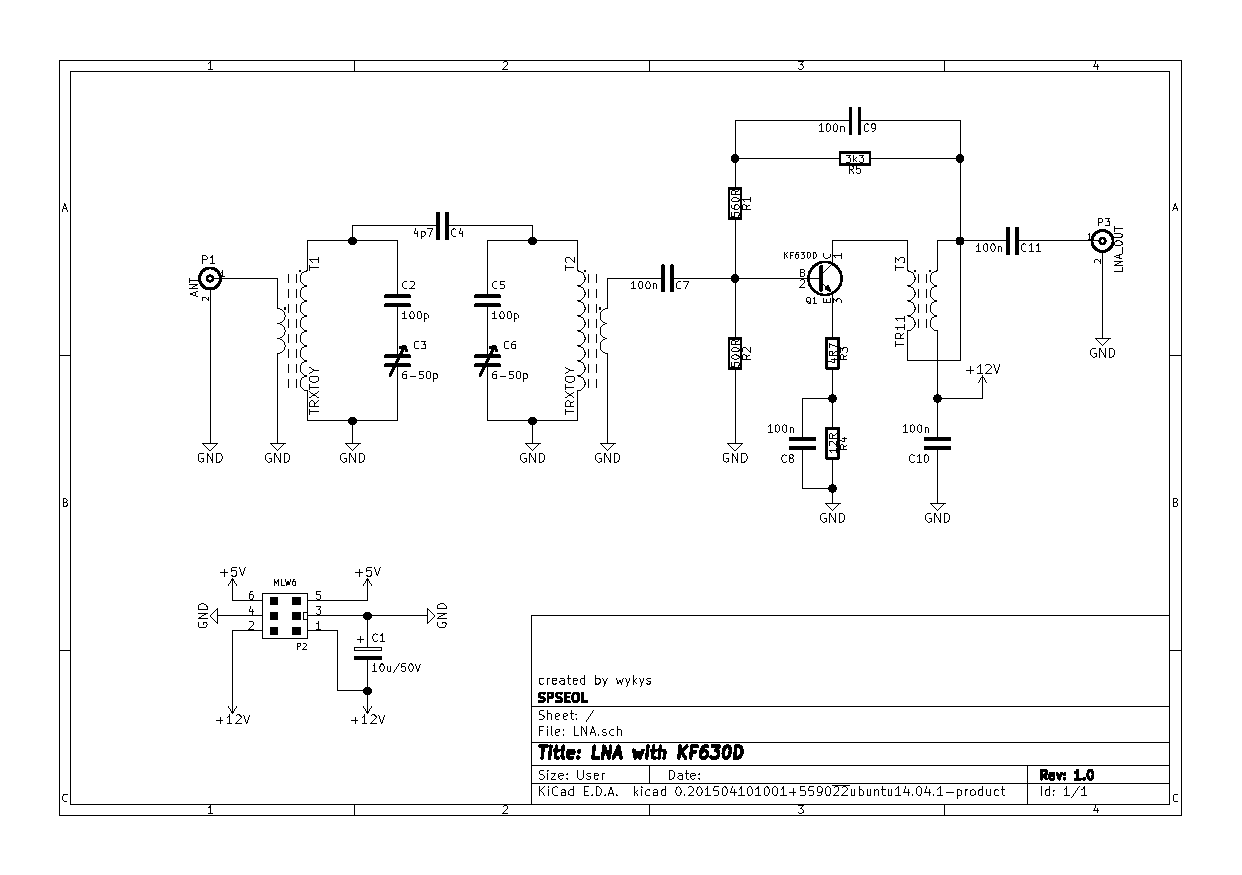
\includepdf[landscape=true]{img/LNA/sch.pdf}



%\subsection{Deska plošných spojů selektivního zesilovače}
%\indent\indent
%Desky plošných spojů jsou oboustranné.
Deska plošného spoje je zhotovena na oboustranném materiálu FR4. Spodní strana tvoří vlastní vrstvu spojů a na horní straně je rozlitá měď kvůli stínění obvodu.

% DPS
\begin{figure}[H]
	\centering
	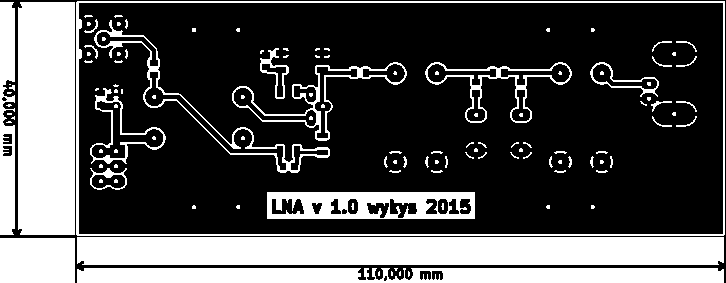
\includegraphics[width=170mm]{img/LNA/cu_b.pdf}
	\caption{Deska plošného spoje selektivního zesilovače, strana spojů}    		
\end{figure}

% os f
\begin{figure}[H]
	\centering
	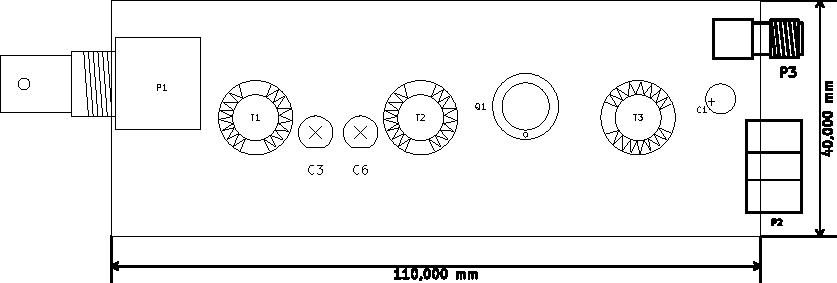
\includegraphics[width=170mm]{img/LNA/os_f.pdf}
	\caption{Osazovací plán selektivního zesilovače, strana součástek}    		
\end{figure}

% os b
\begin{figure}[H]
	\centering
	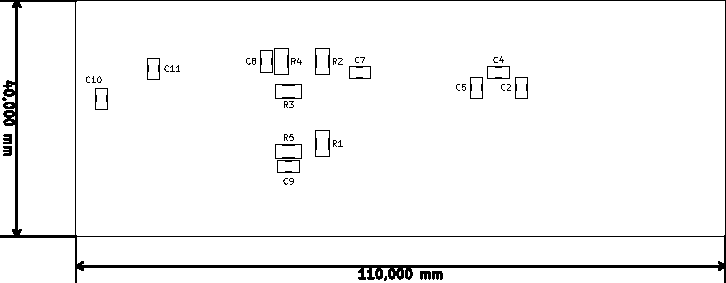
\includegraphics[width=170mm]{img/LNA/os_b.pdf}
	\caption{Osazovací plán selektivního zesilovače, strana spojů}    		
\end{figure}

\begin{table}[H]
	\begin{center}
		\begin{tabular}[H]{!{\vrule width 1pt}c|c|c|c!{\vrule width 1pt}}
		    \specialrule{1pt}{0pt}{0pt} 
		    \textbf{Určovatel}	&	\textbf{Pouzdro}	&	\textbf{Množství}	&	\textbf{Určení}	\\\specialrule{1pt}{0pt}{0pt} 
			T3	&	N2	&	1	&	TR11	\\\hline
			T1,T2	&	Amidon-T44-2	&	2	&	TRXTOY	\\\hline
			C1	&	Elko\_vert\_11x5mm\_RM2.5	&	1	&	10u/50v	\\\hline
			C2,C5	&	C\_0805	&	2	&	100p	\\\hline
			C3,C6	&	CT	&	2	&	6-50p	\\\hline
			C4	&	C\_0805	&	1	&	4p7	\\\hline
			C7,C8,C9,C10,C11	&	C\_0805	&	5	&	100n	\\\hline
			P1	&	BNC&	1	&	ANT	\\\hline
			P2	&	MLW6	&	1	&	napájení	\\\hline
			P3	&	MCX	&	1	&	LNA\_OUT	\\\hline
			Q1	&	TO5	&	1	&	KF630D	\\\hline
			R1	&	R\_1206	&	1	&	560R	\\\hline
			R2	&	R\_1206	&	1	&	500R	\\\hline
			R3	&	R\_1206	&	1	&	4R7	\\\hline
			R4	&	R\_1206	&	1	&	12R	\\\hline
			R5	&	R\_1206	&	1	&	3k3	\\\hline
			M1,M2,M3,M4	&	M3	&	4	&	M3	\\\specialrule{1pt}{0pt}{0pt} 
		\end{tabular}

		\caption{Tabulka použitých součástek pro desku selektivního zesilovače}
		\label{tab:s1}      
	\end{center}
\end{table}
